\input{Preamble_CV.tex}

%%% Begin Document
\begin{document}
% \begin{wrapfigure}{r}{0.3\textwidth}
% 	\vspace*{-0.5cm}
%   \hfill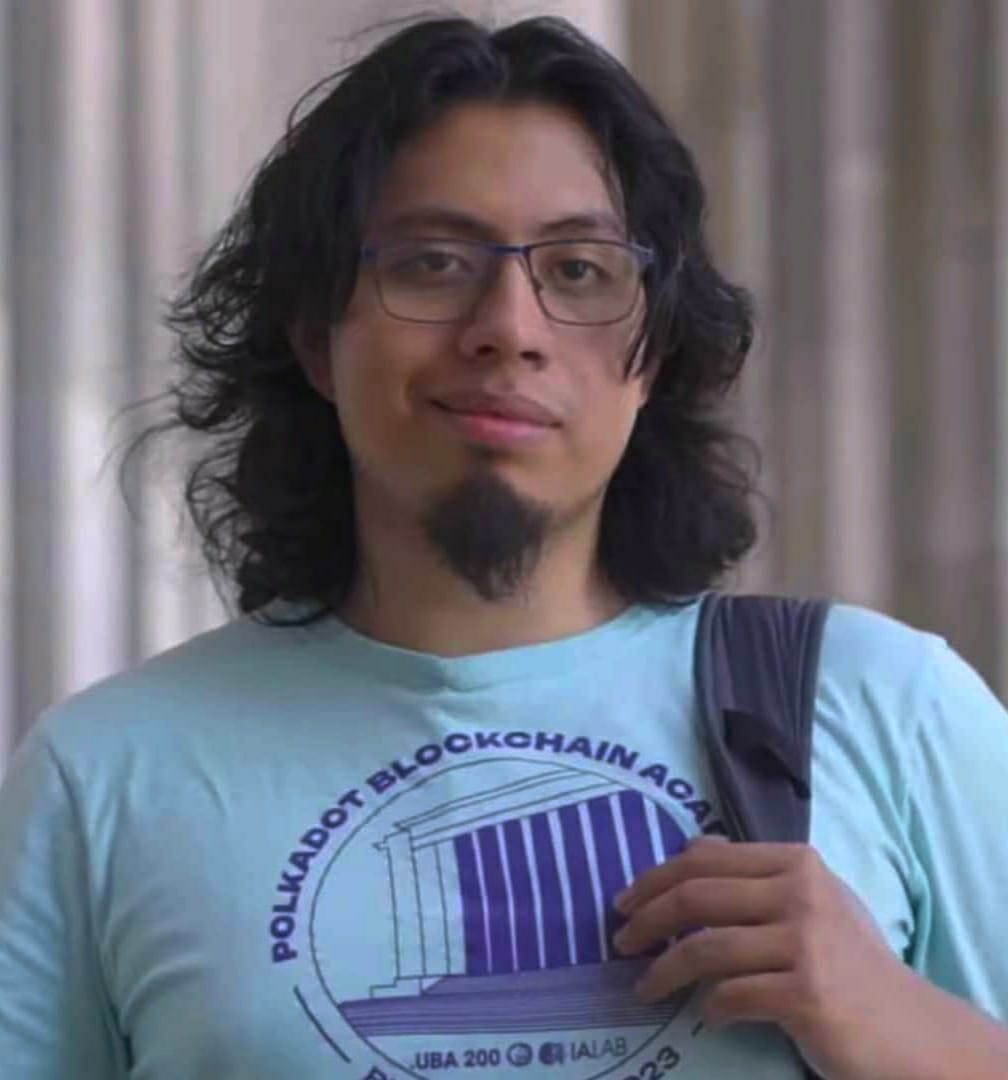
\includegraphics[width=0.2\textwidth]{photo2.jpeg}
% 	\vspace{-5cm}
% \end{wrapfigure}
\MyName{Daniel S\'anchez Dom\'inguez}
\SimpleEntry{\textbf{\Large{Software Engineer}}}
\sepspace

%%% Personal details
%\NewPart{Personal details}

\SimpleEntry{(+52) 811 84 71 700}
\SimpleEntry{\href{mailto:amaniel2718@protonmail.com}{amaniel2718@protonmail.com}}
\TitleEntry{\inlineimg{icons/github.png} Github}{\href{https://github.com/DanEscher98}{DanEscher98}}
\TitleEntry{\inlineimg{icons/linkedin.png} LinkedIn}{\href{https://www.linkedin.com/in/danyiel-colin}{Danyiel Colin}}

\sepspace
\SimpleEntry{
Experienced Software Engineer with +3 years specializing in backend
development. Enthusiastic about mentoring and sharing knowledge with team
members. Thrives in collaborative environments that encourage idea exchange.
Possesses a research-oriented mindset, particularly drawn to abstract
mathematics and functional programming.}

\NewPart{Professional experience}

\TimeEntryFocus{16.Oct.2023 - Dic.2023}{Automation project for RISTOC}{}
{Project to automate the workflow of an online automotive parts store. The developed
components were: a \textbf{PostgreSQL} database, backend logic in
\textbf{Python}, Shopify integration and automated workflows with \textbf{Zapier}.}

\TimeEntryFocus{Jul.2023 - Dic.2023}{CriptoMx Guardian Protocol}{Blockchain Developer}
{Working at the design of smart contracts in \textbf{Rust} to implement a
liquidity staking protocol in the \textbf{VARA} network using the \textbf{GEAR} framework. }

\TimeEntryFocus{Apr.2023 - ...}{Freelancing projects}{}
{Working to develop a basic cybersecurity toolchain (a Fuzzer and Static
Analyzer) for analyzing vulnerabilities in WASM binaries used in \textbf{Ink!}
smart contracts. Utilizing \textbf{Rust} for the implementation.}

\TimeEntryFocus{15.Jan.2022 - 19.Dec.2022}{\inlineimg{icons/johndeere.png} John Deere}{Embedded Systems Engineer}
{Worked in an Agile team using Linux, Python, C, and ARM.
  Accomplishments include: desig and implementation of a kernel driver
  for communication between a processor and a microprocessor through UART and the IOP protocol,
  developing a Python CLI app for booting only USBs with verified ISO images in Windows,
  solving build issues in Jenkins,
  and implementing a RTOS module to convert CAN to Bluetooth,
  taught a series of courses on \textbf{Rust} and its application in embedded systems. }

\TimeEntryFocus{Summer 2022}{\inlineimg{icons/abclog.png} ABC Logistica}{Consultant Web Developer}
{Contracted to document and implement tests in PHP using the Laravel framework.
  Worked with languages like SQL and JavaScript.}


\sepspace
%%% Academic Activities
\NewPart{Academic Activities}
% \TimeEntryFocus{02-11.2009}{Piano course}
% {taught by María Isabel García López}{}
 
% \TimeEntryFocus{Autumn.2011}{Mini Robótica para Adolescentes}
% {program taught by ITESO}{}

\TimeEntryFocus{20-23.Sep.2023}{Hackaton Cripto México Tijuana}{: 3er place}
{Developed a functional MVP of a \textbf{Liquidity Stake} over the \textbf{VARA}
network. The \textbf{smart contracts} were programmed in \textbf{Rust}.}

\TimeEntryFocus{17.Aug.2023}{Rust Instructor in a Workshop at CryptoLatin Fest}{: (Colombia)}
{Conducted a workshop targeting developers interested in learning \textbf{Rust}
and writing smart contracts with \textbf{Ink!}.}

\TimeEntryFocus{07.Jun.2023}{\inlineimg{icons/Ibero.png} Rust Instructor in a Workshop at Univ. Iberoamericana}{}
{Workshop oriented to university students, focused to teach them solid foundations
on \textbf{Rust} and writing smart contracts with \textbf{Ink!}.}

\TimeEntryFocus{10-22.Nov.2020}{\inlineimg{icons/igem.png} iGEM Competition}{: Gold medal}{
  Modification of a bacterium for the expression of ranaspumins, a thermo-resistant protein, 
  for producing fire-fighting foam.}

\TimeEntryFocus{Summer 2020}{X Escuela de Verano Virtual de Matemáticas}{organized by \textbf{UNAM}}{
  Focus on numerical methods to model pandemic dynamics using Python}

\TimeEntryFocus{01-04.Nov.2019}{\inlineimg{icons/igem.png} iGEM Competition}{: Bronze medal (Boston, USA)}{
Designed genetically engineered bacteria for digesting toxic compounds.
Used Python for numerical simulations and cluster computing.
Created an online wiki to document the project.
Presented the project at the iGEM competition in Boston, USA.}

\TimeEntryFocus{Autumn 2019}{Túnel de la biología sintética}{}{Scientific
divulgation activity in which highschoolers were taught about biotechnology
through workshops and interactive stands}

\TimeEntryFocus{Autumn 2019}{Program: CON-CIENCIA UANL}{Participation as organizer}{
  Program to promote STEM skills aimed at low-income high school students.
  Conducted a course on programming concepts and digital electronics.}

\TimeEntryFocus{04-20.Sep.2019}{Course: Biotecnología de Cianobacterias y Microalgas}{: \textbf{FCB-UANL}}
{Hands-on workshop  aimed to learn how to extract microalgae, cultivate
cyanobacteria and count organisms under a microscope.}

\TimeEntryFocus{Summer 2019}{Course: Biotecnología Aplicada a Biomedicina Molecular}{: \textbf{CIDEB-UANL}}
{Hands-on course to learn DNA extraction techniques, protein purification, and
identification of diseases through molecular techniques.}

\sepspace

%%% Education
\NewPart{Education}
\TimeEntryFocus{Jan.2023-Feb.2023}{\inlineimg{icons/Polkadot.png} Polkadot Blockchain Academy}{: \textbf{Parity} x \textbf{UBA} (Argentina)}
{An in deepth course, research oriented, working with core libraries of the \textbf{Substrate} framework in \textbf{Rust}}

\TimeEntryFocus{2018-2022}{\inlineimg{icons/fime.png} University studies as Network Engineer}{: \textbf{UANL} (Mexico)}
{Focused on systems programming and embedded development}

\TimeEntryFocus{Autumn 2020 - Summer 2021}{\inlineimg{icons/Qiskit-Logo.svg.png} The Coding School’s Qubit by Qubit}{: \textbf{IBM}}
{Completed a two-semester Quantum Computing course using the \textbf{Qiskit} framework}

\TimeEntryFocus{Spring 2022}{\inlineimg{icons/cardano.png} Plutus Pioneers 3rd Cohort}{: \textbf{IOHK}}
{Completed a hands-on course using \textbf{Haskell} to learn about the Cardano Blockchain and Smart Contracts development.}

	%Average to date: 5\\
	%Expected graduation in June of 2024}


%%% Skills and Qualifications
\NewPart{Skills and Qualifications}
\NewSubPart{Languages}
\SimpleEntry{\textbf{Native}: Spanish, \textbf{C1}: English, \textbf{A2}: French}

\NewSubPart{Programming Languages}
\SimpleEntry{
\textbf{Advanced}:
\inlineimg{icons/rust.png} Rust,
\inlineimg{icons/python.png} Python,
\inlineimg{icons/C_lang.png} C,
\inlineimg{icons/bash.png} Bash;
\textbf{Intermediate}:
\inlineimg{icons/haskell.png} Haskell,
\inlineimg{icons/laravel.png} PHP/Laravel}

\end{document}
